As a final set of calculations with pure neutron matter, we can look at performing CC calculations using the CCD(T) approximation.

%% CCD(T) DATA
First, let us compare the correlation energies of a PNM system for densities around nuclear density calculated using CCD, CCDT-1, and CCD(T).  It has already been shown that CCD and CCDT-1 give significantly different values for the correlation energies. Still, we want to ensure a significant difference between these two data sets and the CCD(T) energies. Fig. \ref{fig:compare_pnm_all_no_sre} shows the fully converged correlation energies for a PNM system calculated with the three CC approximations.  The CCD and CCD(T) were performed at M = 1,478, and the CCDT-1 calculations were performed at M = 514.  It does appear that the three methods give significantly different answers, so it will be an exciting test for the SRE method to compare its performance on all three methods.

\begin{figure}
    \centering
    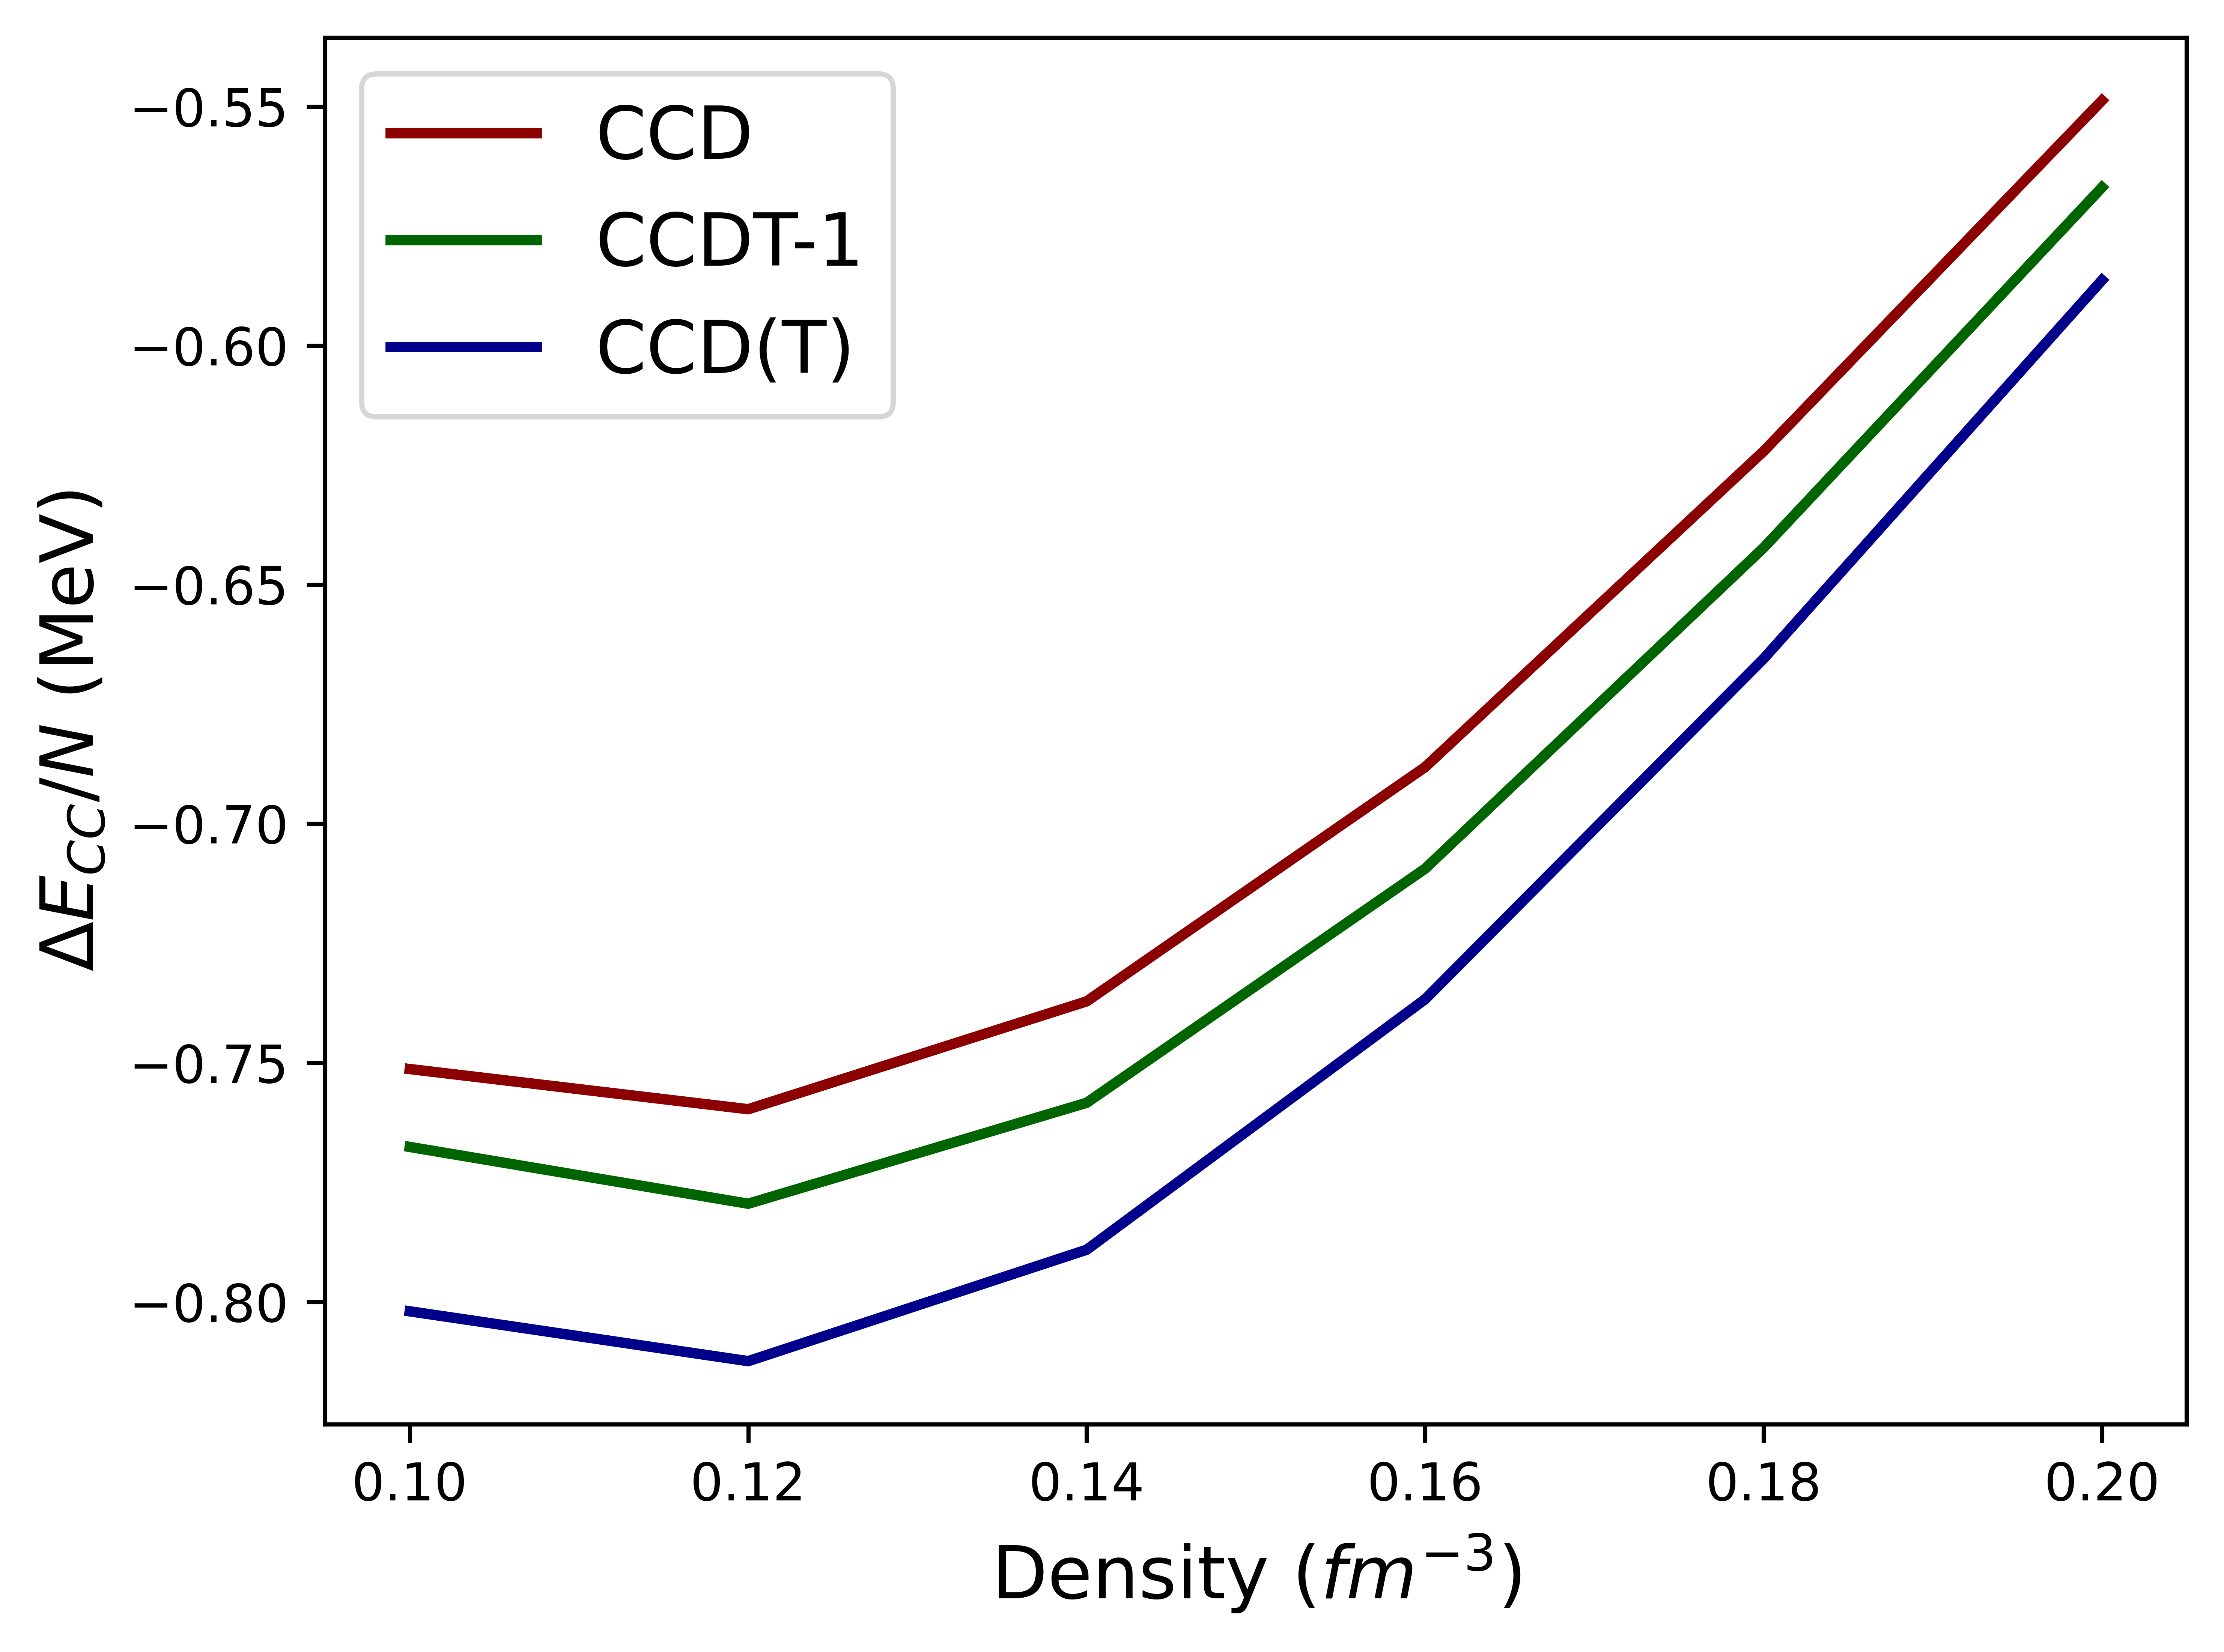
\includegraphics[scale=0.75]{Images/Chapter8/pnm_all_sre.png}
    \caption{Correlation energies of PNM calculated with CCD (red), CCDT-1 (green), and CCD(T) (blue) for densities around nuclear density.}
    \label{fig:compare_pnm_all_no_sre}
\end{figure}

Now, we can compare the run times of each method when applied to PNM.  The expected run time of a CCD calculation is an iterative $O(M^6)$, and the expected run time of a CCDT-1 calculation is an iterative $O(M^7)$.  In comparison, the expected run time of a CCD(T) calculation falls in between these two with an iterative $O(M^6)$ followed by a non-iterative step of $O(M^7)$.  And in fact, that is what we see in Fig. \ref{fig:all_times_pnm} where CCD(T) is faster than CCDT-1 but slower than CCD. Note that the times are reported here in node hours per GHz.  The CCD(T) calculations for PNM were performed on Oak Ridge National Laboratory's Andes supercomputer on Andes processors, which have a clock speed of 3.0 GHz and use 64 MPI nodes.  Just as we defined a node hour as the total run time of a calculation multiplied by the number of MPI nodes in the calculations to compare the run times computed with different numbers of MPI nodes, here we define node hours per GHz (node hours divided by the clock speed of the processors) to compare results which have been performed on different supercomputers. 

\begin{figure}
    \centering
    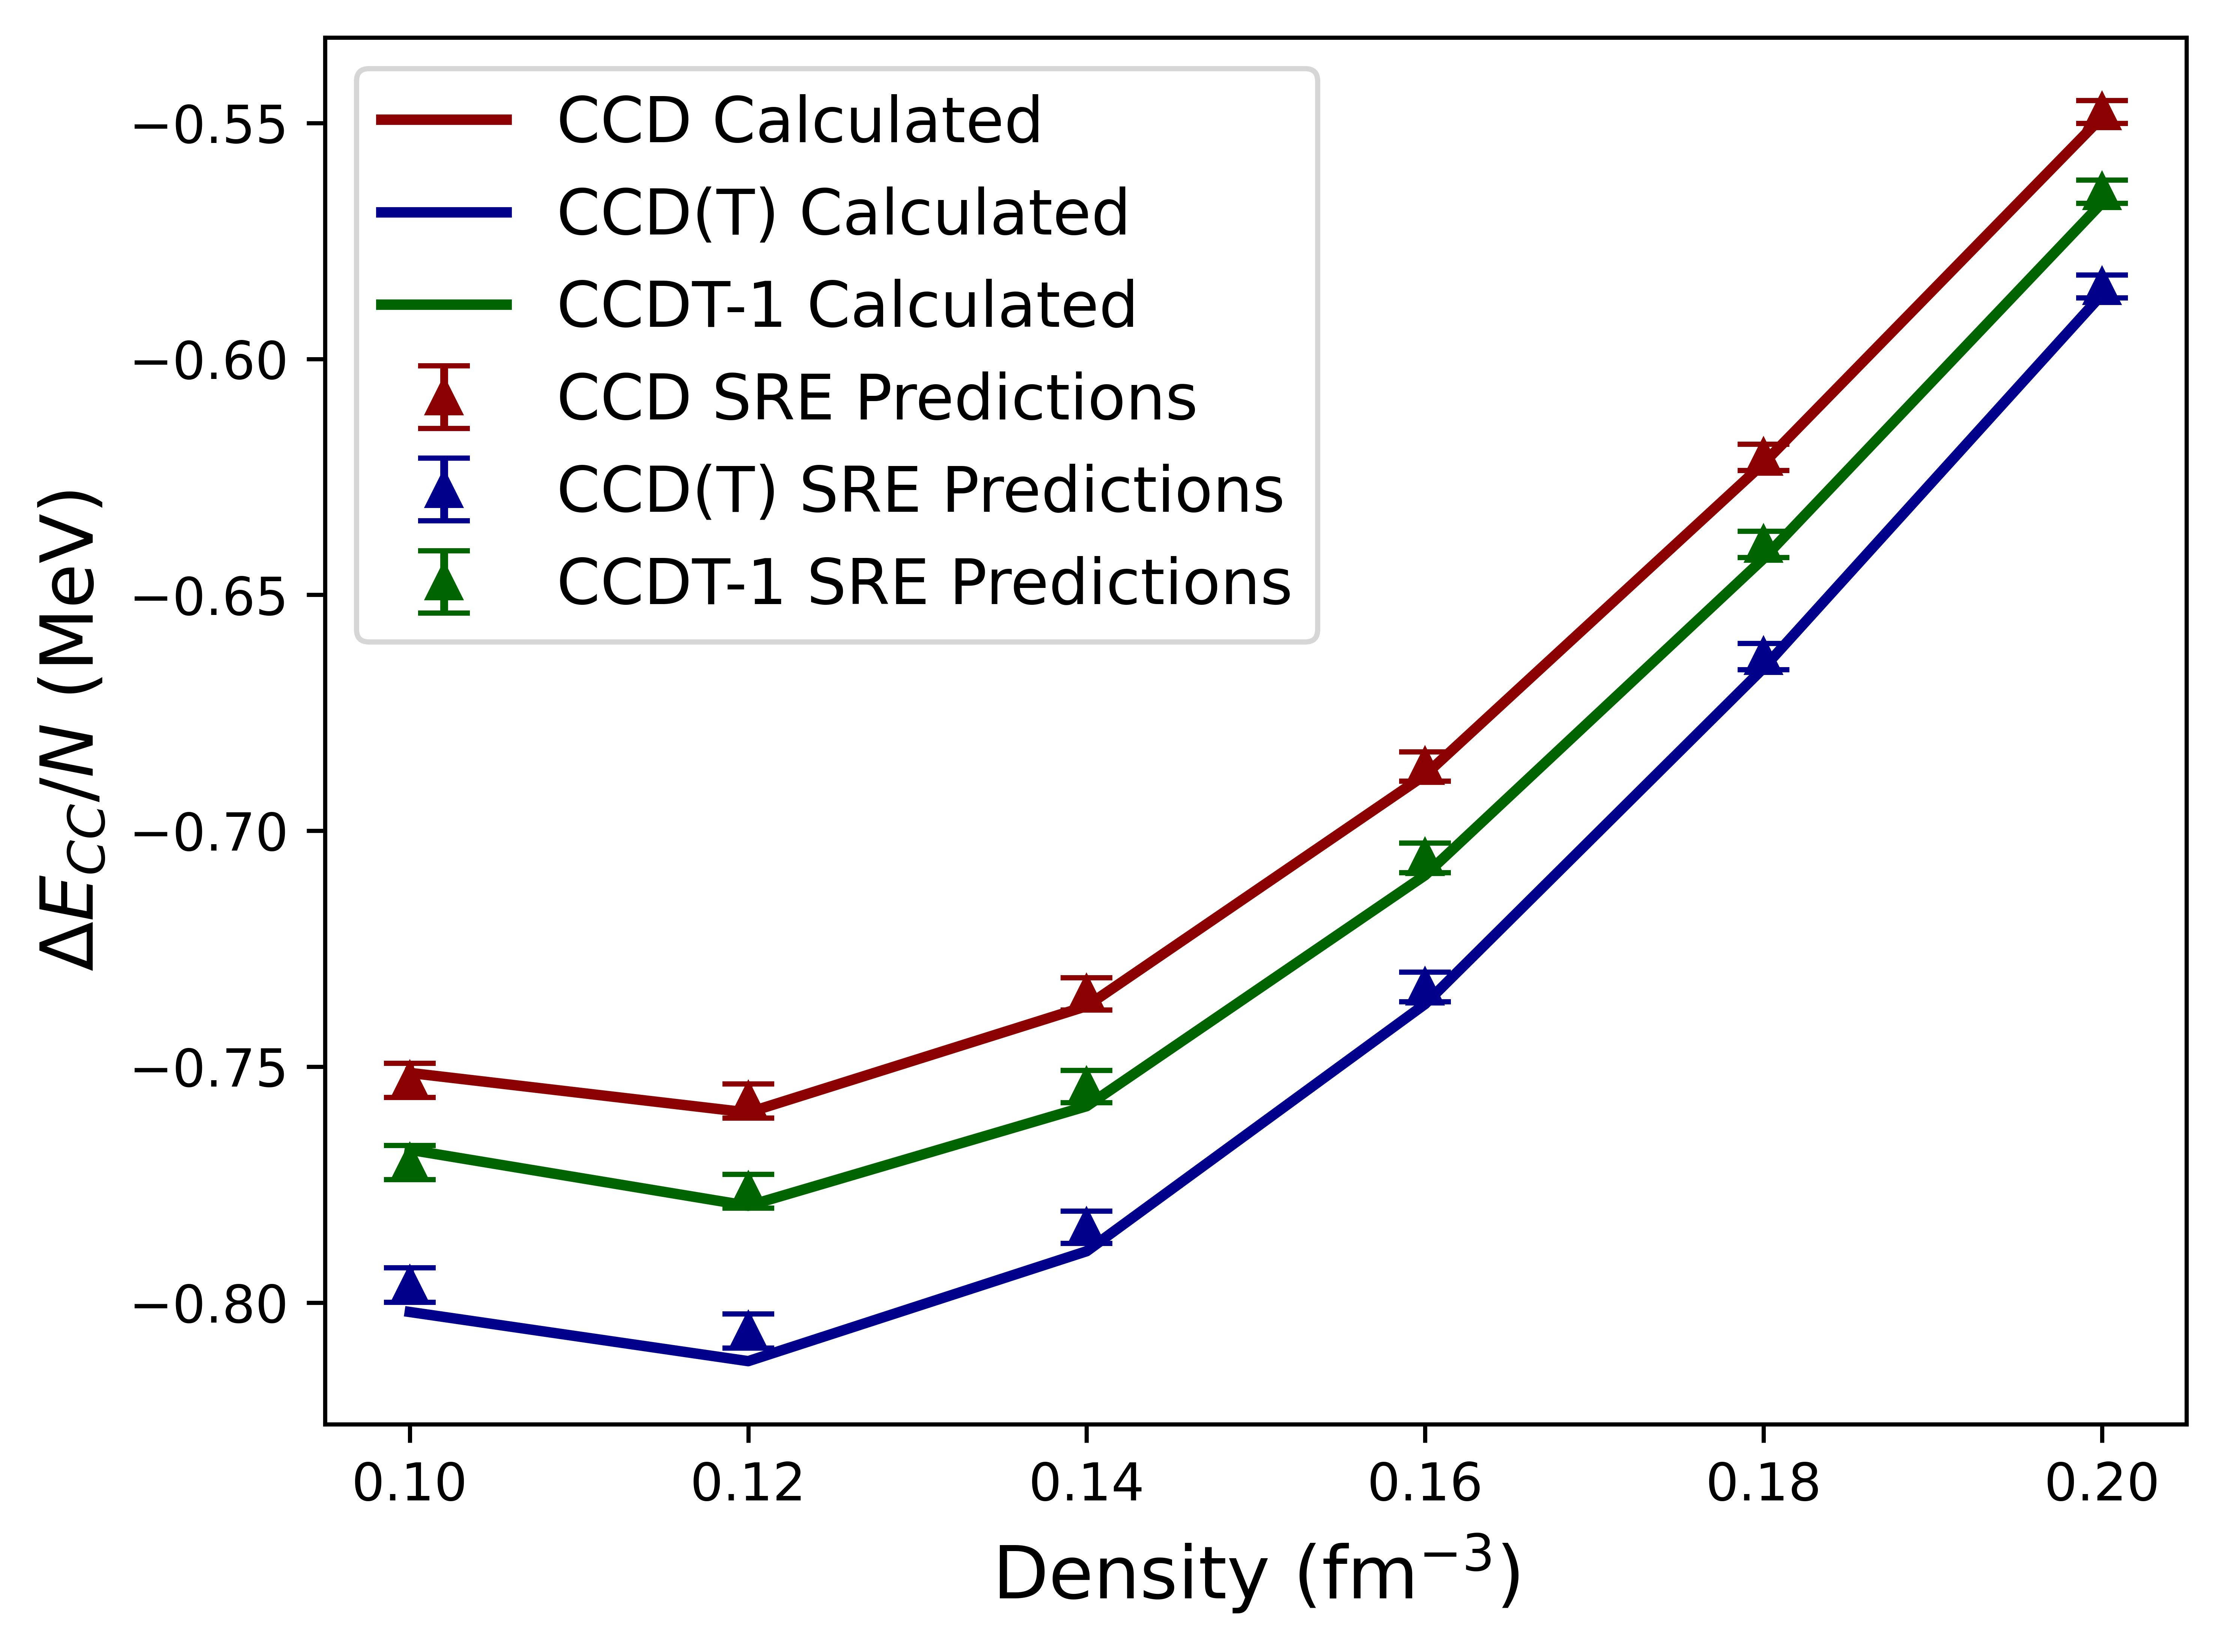
\includegraphics{Images/Chapter8/FinalReport6.png}
    \caption{The run time (in node hours per GHz) to calculate the correlation energies for a PNM system at d = 0.16fm$^{-3}$ calculated using CCD (red), CCDT-1 (green), and CCD(T) (blue) as a function of the number of single-particle states in the calculation.}
    \label{fig:all_times_pnm}
\end{figure}

Now we can apply the SRE method to attempt to predict the converged CCD(T) correlation energies for PNM.  We have used three training points, like with the other PNM and chiral potential extrapolations. Still, here we have moved the training data to slightly higher numbers of single-particle states (M = 186, 246, and 294) due to the slower convergence of the CCD(T) correlation energies with respect to the number of single-particle states.  We have kept the SRE sequence length as 1.  Fig. \ref{fig:sre_pnm_ccdt_pert} shows the results of performing this SRE analysis with the full CCD(T) correlation energy calculations performed at M = 1,478 shown with the solid line and the SRE predictions with the triangular markers.  Here the average percent error between the two data sets is 0.54$\%$.  Furthermore, the time needed to perform the six CCD(T) calculations at M = 1,478 shown in Fig. \ref{fig:sre_pnm_ccdt_pert} took 594.15 node hours, but the time needed to generate the SRE training data was only 32.16 node hours.  This leads to a time savings of 561.99 node hours or 23.41 \textit{node days}.

\begin{figure}
    \centering
    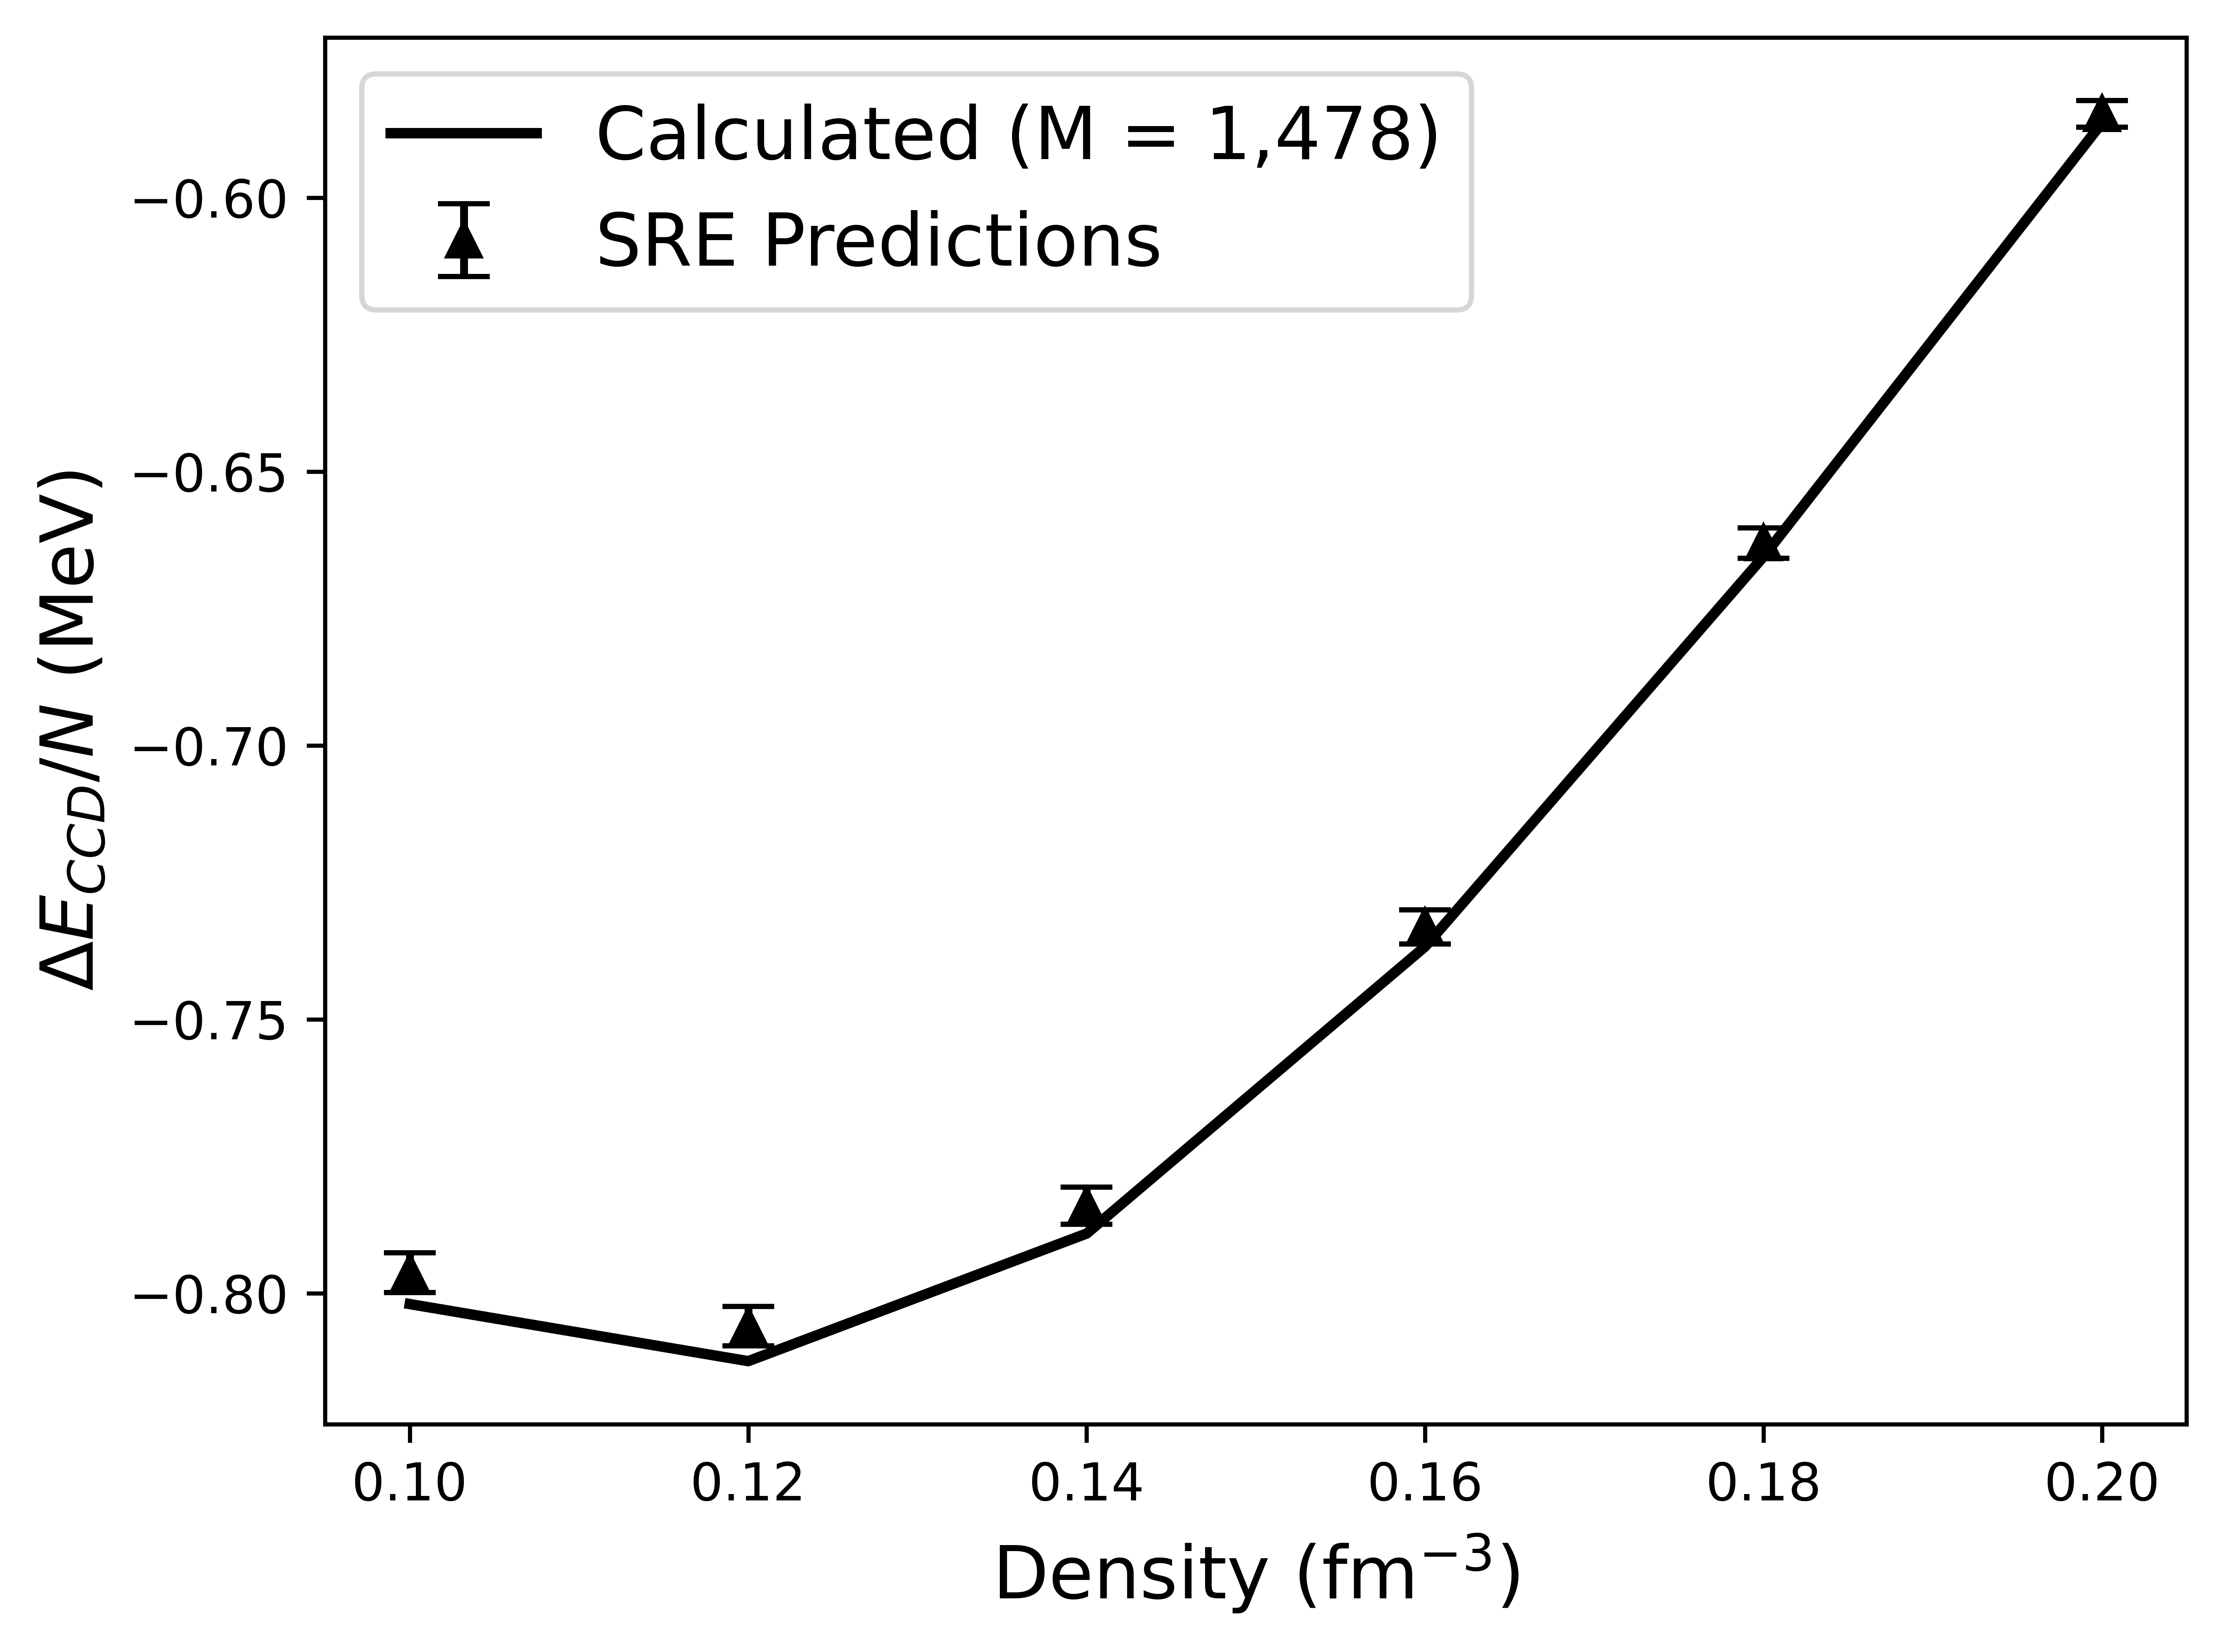
\includegraphics{Images/Chapter8/FinalReport4a.png}
    \caption{The CCD(T) correlation energies for PNM for densities around nuclear density were calculated at M = 1,478 (solid line) and predicted with the SRE method (triangular markers).  The uncertainties from the Gaussian processes algorithm are shown with error bars on the markers.}
    \label{fig:sre_pnm_ccdt_pert}
\end{figure}


Finally, we are in a position to compare the SRE predictions for CC calculations of PNM using CCD (red), CCDT-1 (green), and CCD(T) (blue), as seen in Fig \ref{fig:compare_pnm_all_sre}.  For all three CC methods, the complete calculations are shown with solid lines. The SRE predictions are shown with triangular markers with error bars, with the error bars representing the uncertainties from the Gaussian processes algorithm. For all three data sets, the SRE method appears to provide a good match for all the correlation energies across all the densities shown.  The average percent error of this figure is 0.42$\%$.  Furthermore, the entire time saved u
using the SRE method to predict the converged correlation energies rather than fully calculating them is 796.89 node hours or 33.20 \textit{node days}.  Therefore, in calculating just 18 points for the PNM system, we save over a month of computational time using the SRE method. 

\begin{figure}
    \centering
    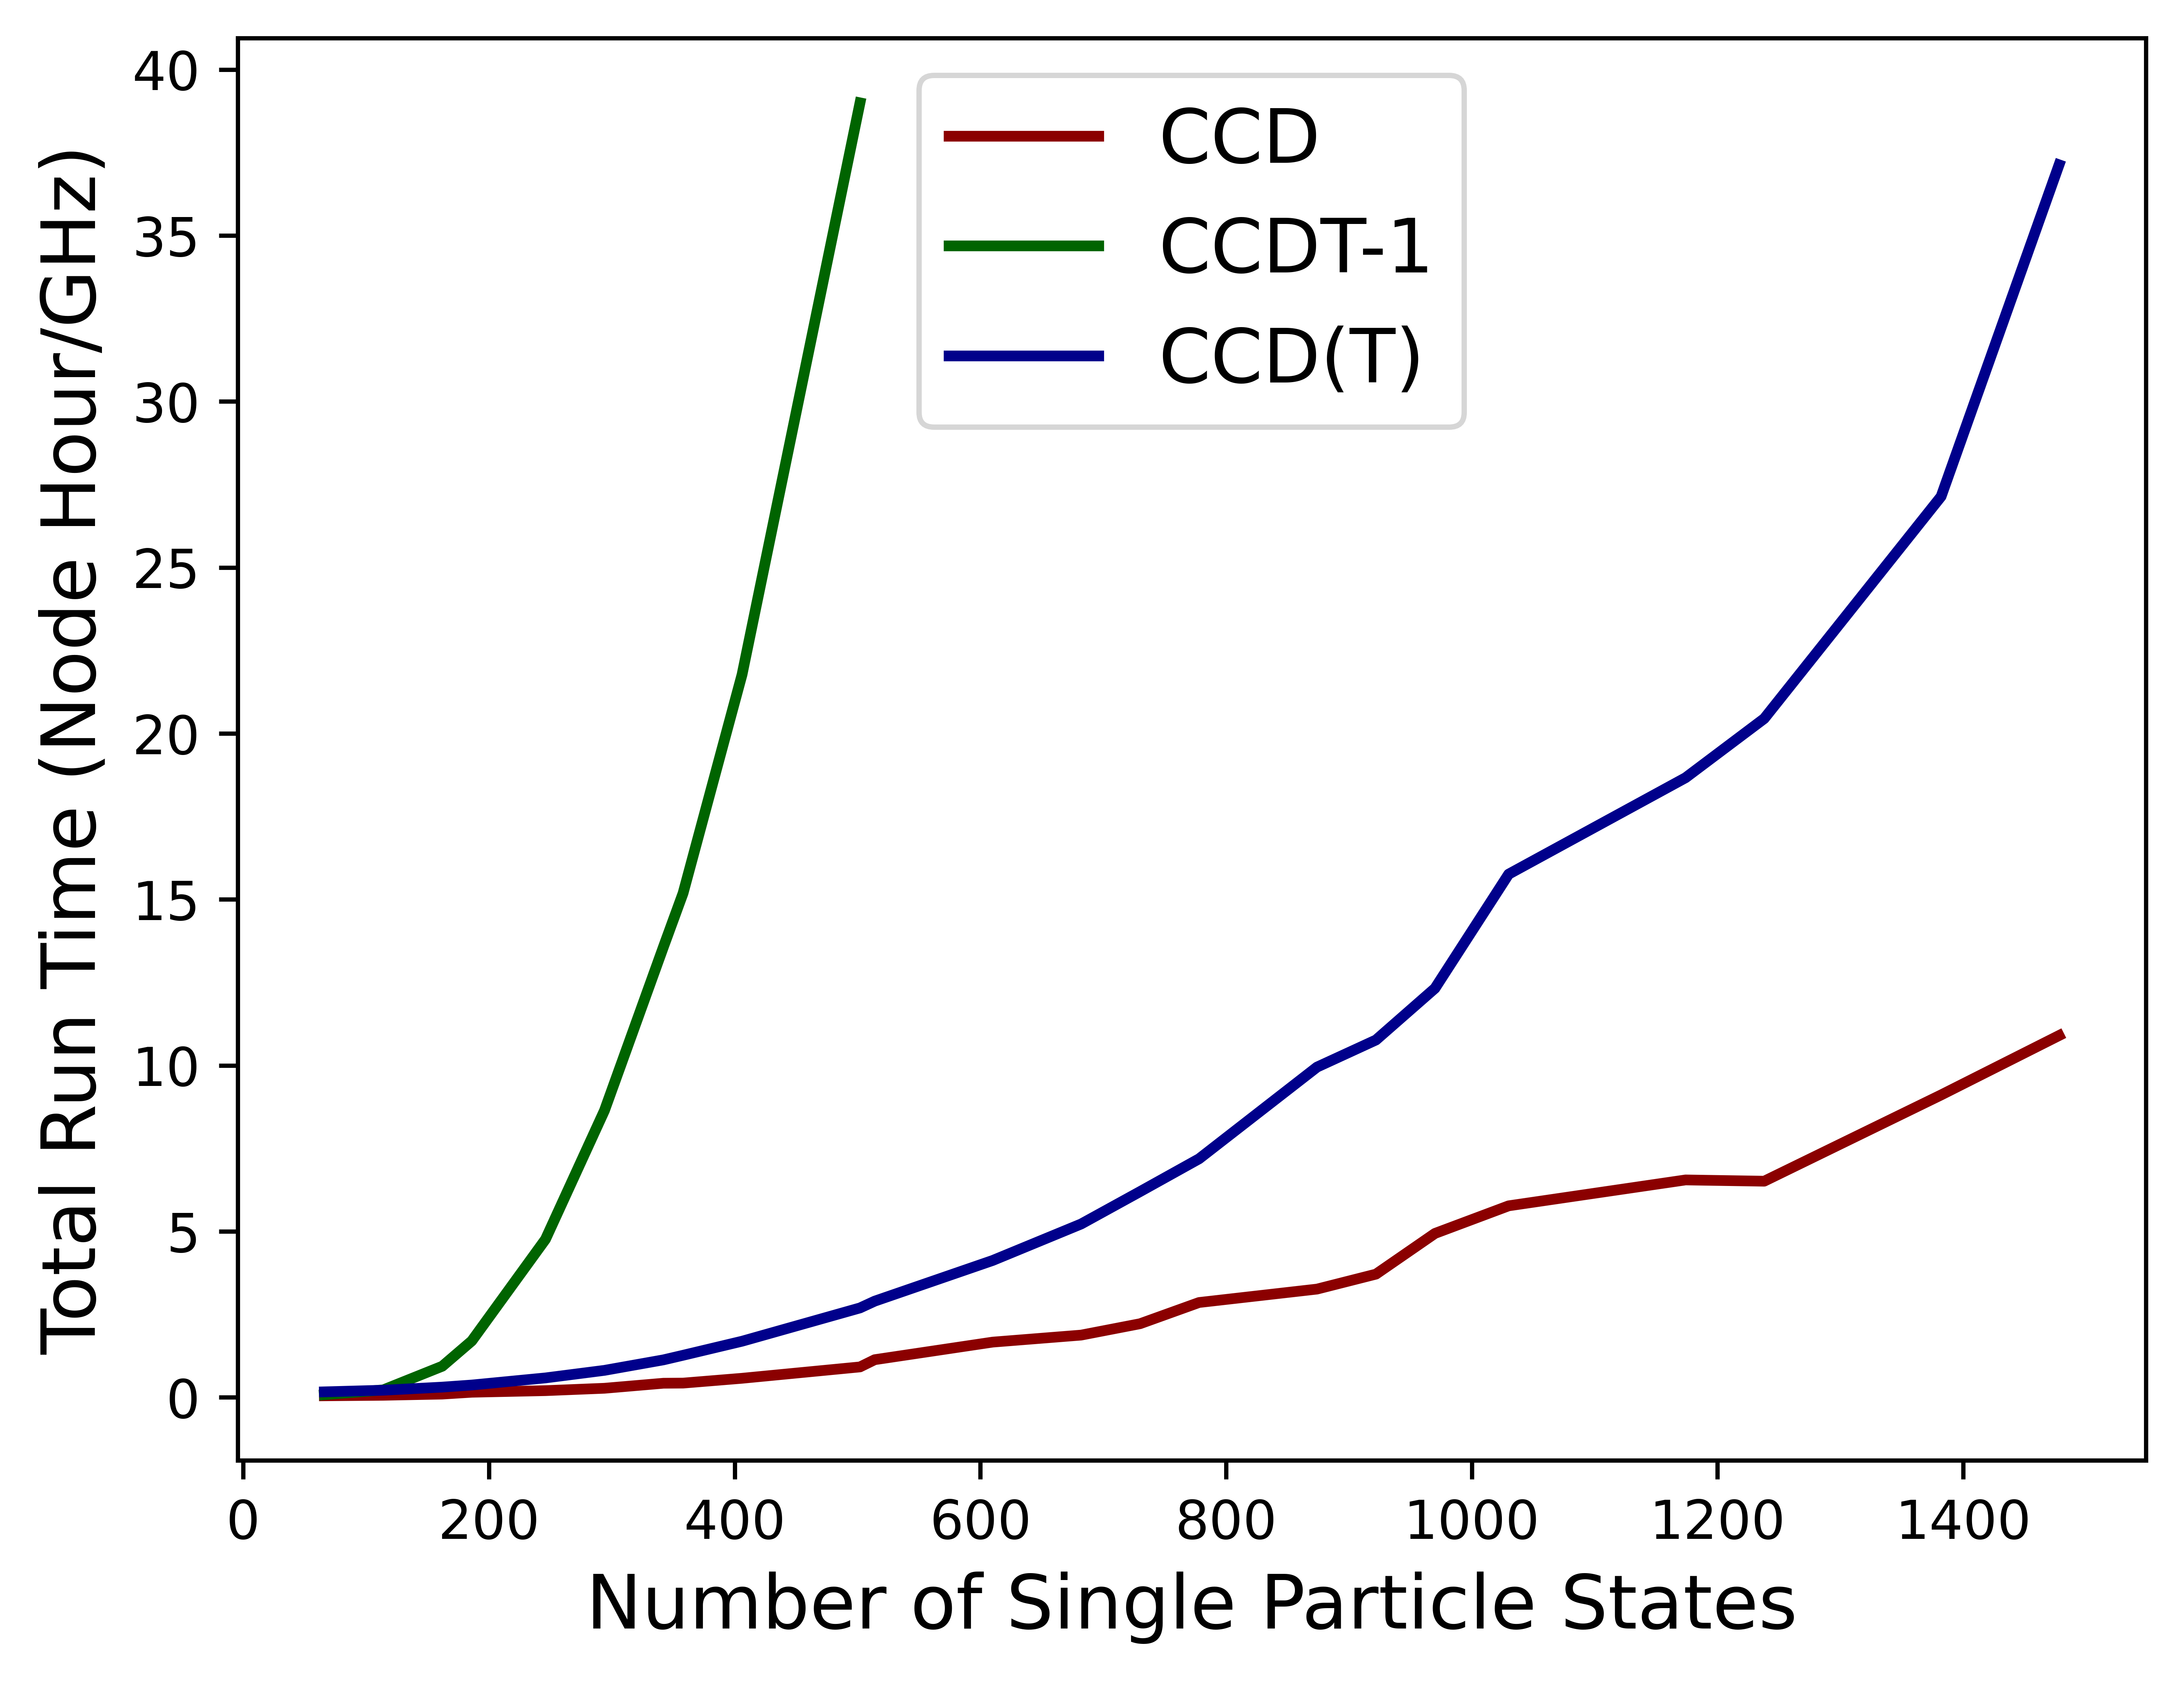
\includegraphics{Images/Chapter8/FinalReport7.png}
    \caption{The correlation energies for PNM were calculated using CCD (red), CCDT-1 (green), and CCD(T) (blue).  The fully converged calculations are shown with the solid lines, and the SRE predictions are shown with the triangular markers.}
    \label{fig:compare_pnm_all_sre}
\end{figure}

In this section, we have performed coupled cluster calculations of pure neutron matter using two different models of nuclear interaction and three different levels of coupled cluster approximations.  However, it is essential to note that the main point of this section is not to compare the effects of different coupled cluster calculations and interactions, though we have done this.  Instead, the main point of this section is to determine the performance of the SRE methods on different types of coupled cluster calculations.  As we have seen throughout this section, the SRE method can accurately extrapolate to the converged correlation energy of the pure neutron matter system, regardless of the combination of nuclear interaction and coupled cluster approximation used. Furthermore, over a month of computational time is saved in this section by using the SRE method with no loss of relevant accuracy. Finally, it is essential to note that even though we are using machine learning, the training data sets we have used range from 3 - 10 data points. These are some of the smallest training data sets found in the literature for machine learning applications in the physical sciences and emphasize an essential feature of the SRE method.  That being that the SRE method can make very accurate extrapolations using very little training data..